\section{Introduction}

With the rapid increase in technology involved in images, there is great needs to establish efficient  algorithms for what is known as salience detection, that is,finding regions or object of interest in an image.The human brains can perform this detection very quickly, and doing so on a computer is a great task for researchers and scientists.This problem is related to image cropping, object recognition and image cropping.Mostly researchers divide this problem into two category.One is global scheme and local scheme.In local scheme a salient region is calculated with respect to it's local region in an image whereas global scheme give priority to when a region is distinct with respect to the whole region of an image.There are some other methods where researcher combined these global and local scheme to get salient region of an image.

\subsection{Local and Global Approaches}
Bottom-up approaches focuses on cues that we naturally interested in, like colors, orientation, density and frequency  

\begin{description}
  \item[$\bullet$]Itti, Koch and Niebur\cite{itti1998model}   proposed a visual attention
  model in which image features such as color, intensity, and
orientation for LDR images are combined to form a single saliency map.It makes use of Gaussian based approach in
which a Gaussian pyramid is formed in each channel by subsampling the input image.Each feature is computed by a set of linear centre-surround operations. Centre-surround is implemented in the model as the difference between fine and coarse scales. The across-scale subtraction is obtained by interpolation to the centre scale and point-by-point
subtraction. Afterwards, all feature maps are combined into a “conspicuitymap” in each channel. Conspicuity maps from all channels one master saliency map, which topographically represents the local saliency.


\item[$\bullet$] Sidib{\'e}, D{\'e}sir{\'e} and M{\'e}riaudeau\cite{sidibe2016visual}  proposed saliency  based on the common observation
that local salient regions exhibit distinct geometric and texture patterns
from neighbouring regions. The colour distribution of local image
patches is modelled with a Gaussian density and measure the saliency
of each patch as the statistical distance from that density.


\begin{figure}[h!]
  \centering
  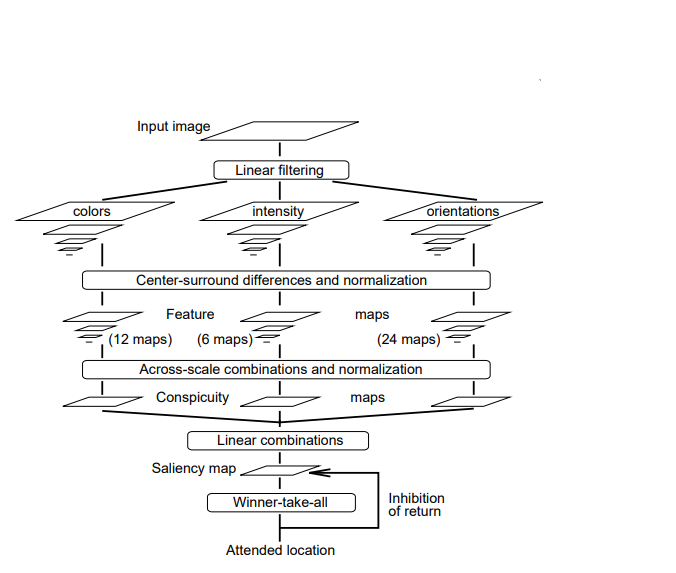
\includegraphics[width=1\textwidth,height=1\textwidth]{pictures/figure1.png}
  \caption[]{Framework of visual attention for Rapid Scene Analysis \cite{itti1998model}}
  \label{orangeleaf}

\end{figure}

\item[$\bullet$]Nevrez mamolu, Weisi Lin, and Yuming Fang \cite{imamoglu2013saliency} 
suggested a saliency detection model in which image is
represented as quaternionic and developed a multiresolution
spatiotemporal saliency detection model called phase
spectrum of quaternion Fourier transform (PQFT) to compute
the spatiotemporal saliency map from the images quaternion
representation. First, each pixel of the image is represented by
a quaternion that consists of color, intensity and motion
feature. Then, the phase spectrum of QFT is used to calculate
the spatiotemporal saliency map, which considers not only
salient spatial features like color, orientation and others in a
single frame but also temporal feature between frames like
motion.

\item[$\bullet$] Qinmu Peng, Yiu-ming Cheung and Xingeand Yuan \cite{peng2017hybrid} , presents a visual saliency detection approach,
which is a hybrid of local feature-based saliency and global
feature-based saliency. First, for a given input image, use an
automatic selection of smoothing parameter scheme to make
the image region more homogeneous. Then, partition the
smoothed image into a set of regions and compute the local
saliency by measuring the color and texture dissimilarity in
the smoothed regions and the original regions, respectively.
Furthermore, compute the global saliency by utilizing the
global color distribution model embedded with color
coherence, together with the multiple edge saliency. Finally,
combine the local and global saliencies, and utilize the
composition information to obtain the final saliency

\begin{figure}[h!]
  \centering
  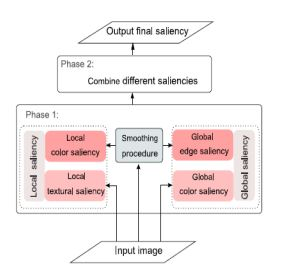
\includegraphics[width=.5\textwidth,height=.6\textwidth]{pictures/figure2.JPG}
  \caption[]{Hybrid of local and global saliency detection\cite{peng2017hybrid}}
  \label{orangeleaf}

\end{figure}


\item[$\bullet$] Yan and Zhi chun \cite{ren2014salient}  presents visual saliency detects which is based on fast bottom-up data driven saliency detection using global contrast method which extracts a large-scale object from background.The global contast based method uniformly
highlighting entire objects is preferred over local contast
based methods which produce high saliency values at or
near object edges. The region based texture contrast is
incorporated into the process of salient map computation
upon the basis of the region based color contrast

\item[$\bullet$] Zhixiang Ren, Shenghua Gao, Liang-Tien Chia\cite{ren2014region}, and
Ivor Wai-Hung Tsang presents a region-based solution for
saliency detection applicable to better encode the image
features for solving object recognition task. First use the
adaptive mean shift algorithm to extract superpixels from the
input image. Then apply Gaussian mixture model (GMM) to
cluster superpixels based on their color similarity. Finally,
calculate the saliency value for each cluster using spatial
compactness metric together with modified PageRank
propagation.

\begin{figure}[h!]
  \centering
  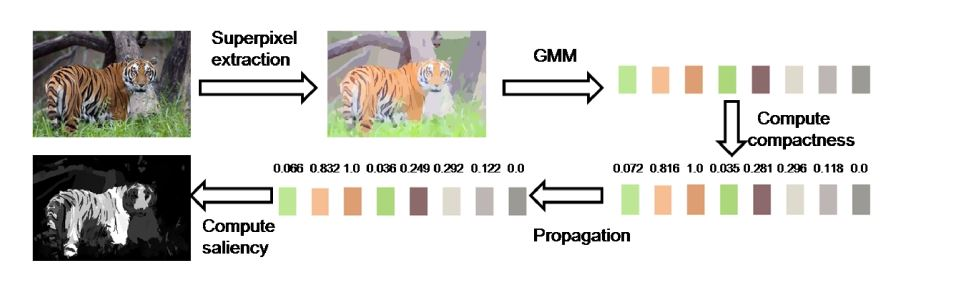
\includegraphics[width=1\textwidth,height=.5\textwidth]{pictures/figure3.jpg}
  \caption[]{Region-Based Saliency Detection\cite{ren2014region}}
  \label{orangeleaf}
\end{figure}

\item[$\bullet$] Zhu, Shuang, Yichen \cite{zhu2014saliency}  propose a robust back-ground measure
called background connectivity.It characterizes the spatial layout of image regions with respect to
image boundaries and is much more robust. It has an intuitive geometrical interpretation and presents unique benefits that are absent in previous saliency measures.Then they propose a principle optimization framework to intregate multiple low level cues including background measure to obtain clean and uniform saliency maps.



\item[$\bullet$] Achanta,R,Hermani\cite{achanta2009frequency}  proposed introduced a frequency tuned saliency detection method. Using the color
differences from the average image color to define pixel saliency.

\item[$\bullet$] Chenlei Guo and Liming Zhang \cite{guo2010novel}  presents a saliency
detection model based on high-pass coefficients of the
wavelet decomposition. The idea is to create the feature maps
by IWT on the multi-level decomposition. First, RGB image
is converted into LAB color space. Then, apply wavelet
transform decomposition on the noise removed version to find
scaling coefficients. In addition to it, it focuses on creating the
feature maps by IWT on the multi-level decomposition. Two
saliency maps are created: local and global saliency maps.
Finally, the local and global maps are combined to yield the
final saliency map. The final saliency map represents both the
local contrast of each location on the scene and the global
distribution of the features as an amplifier for local saliency
values

\item[$\bullet$] Zhi Liu, Xiang Zhang, Shuhua Luo, and Olivier\cite{liu2014superpixel}  proposed a superpixel-based spatiotemporal saliency
model for saliency detection in videos. First, based on the
superpixel representation of video frames, motion histograms
and color histograms are extracted at the superpixel level as
local features and frame level as global features. Then,
superpixel level temporal saliency is measured by integrating
motion distinctiveness of superpixels with a scheme of
temporal saliency prediction and adjustment, and superpixellevel spatial saliency is measured by evaluating global
contrast and spatial sparsity of superpixels. Finally, a pixellevel saliency derivation method is used to generate pixellevel temporal and spatial saliency maps, and an adaptive
fusion method is exploited to integrate them into the
spatiotemporal saliency map.

\begin{figure}[h!]
  \centering
  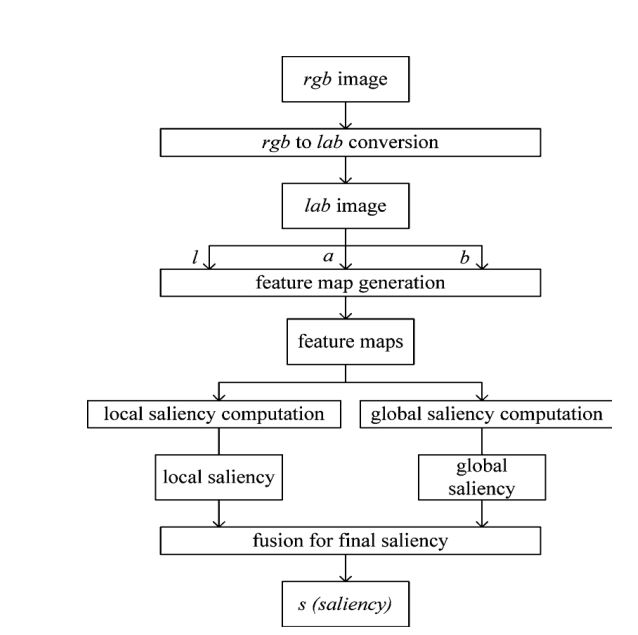
\includegraphics[width=1\textwidth,height=0.9\textwidth]{pictures/figure4.jpg}
  \caption[]{Framework of visual attention for Rapid Scene Analysis \cite{guo2010novel}}
  \label{orangeleaf}
\end{figure}

\item[$\bullet$] Yuanyuan Dong, Mahsa T. Pourazad, and Panos
Nasiopoulos\cite{dong2016human}   proposed a saliency detection method that
detects the saliency of HDR images and HDR video frames.
The spatial and temporal cues are taken into account, leading
to two saliency maps: the spatial saliency map and the
temporal saliency map. First, to obtain the spatial saliency
map, use the HVS model to decompose feature channels from
an HDR input and then follow the procedure of the classical
bottom-up method in \cite{itti1998model}. Then to compute the temporal
saliency map, an optical flow based method is used to
estimate motion. Finally, a dynamic fusion method is
proposed to combine both the spatial and temporal saliency
maps.

\item[$\bullet$]Libio ,Lin and Tiejian \cite{zhang2016unified}  proposed visual saliency based on 
color and texture features and incorporating higher-level priors.The SLIC superpixel algorithm is applied to form an over-segmentation of the image. Color saliency map and texture
saliency map are calculated based on the region contrast method and adaptive weight.
Higher-level priors including location prior and color prior are incorporated into the model to
achieve a better performance and full resolution saliency map is obtained by using the upsampling method. 

\item[$\bullet$] M.M. Cheng et al. \cite{cheng2015global}  presented a regional contrast
based salient object detection algorithm that evaluated global contrast differences and spatial
weighted coherence scores. They used the saliency maps to accomplish unsupervised salient
object segmentation.



\item[$\bullet$] Wonjun Kim, Chanho Jung, and Changick Kim \cite{kim2011spatiotemporal} 
suggested a novel unified method for detecting salient regions
in both images and videos based on a discriminant centersurround hypothesis that the salient region stands out from its
surroundings. First of all, a set of visual features composed of
edge and color orientations and temporal gradients are
computed. Then, compute the spatiotemporal saliency at each
scale in which the spatial saliency is computed as the
distances between ordinal signatures of edge and color
orientations obtained from the center and the surrounding
regions and the temporal saliency, by simply computing the
sum of absolute difference (SAD) between temporal gradients
of the center and the surrounding regions. Finally, resize
saliency map to the same size of input image to obtain the
final saliency.


\end{description}

\section{Conclusion}
In this chapter, we presented the common method for finding visual saliency detection.By previewing various method we learned advantage and disadvantage of various method and their characterstic
for simple and clean visual saliency detection.